% This file was created with tikzplotlib v0.10.1.
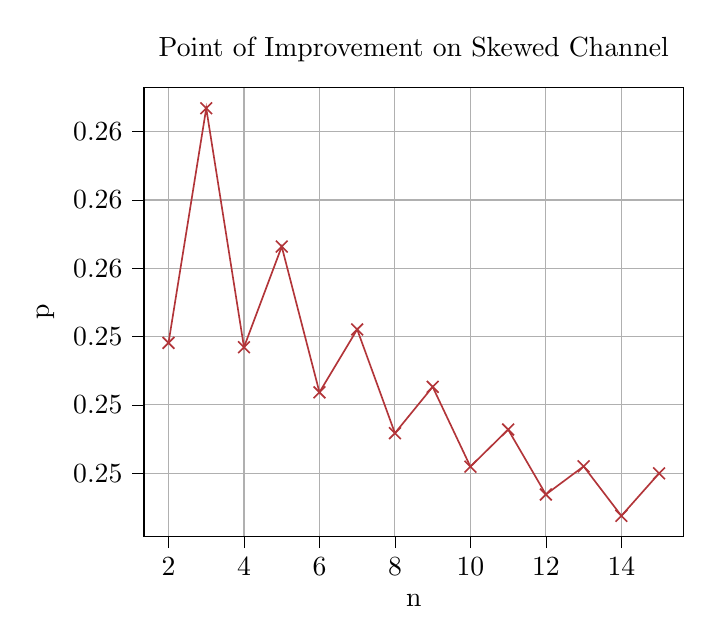
\begin{tikzpicture}

\definecolor{brown1785357}{RGB}{178,53,57}
\definecolor{darkgrey176}{RGB}{176,176,176}

\begin{axis}[
tick align=outside,
tick pos=left,
title={Point of Improvement on Skewed Channel},
x grid style={darkgrey176},
xlabel={n},
xmajorgrids,
xmin=1.35, xmax=15.65,
xminorgrids,
xtick style={color=black},
y grid style={darkgrey176},
ylabel={p},
ymajorgrids,
ymin=0.248151071103398, ymax=0.261286191172616,
yminorgrids,
ytick style={color=black}
]
\addplot [semithick, brown1785357, mark=x, mark size=3, mark options={solid}]
table {%
2 0.253814638739268
3 0.260689140260378
4 0.253687417133649
5 0.256637512471517
6 0.252366398501502
7 0.254208695072492
8 0.25117025275294
9 0.252526759833336
10 0.250189119106293
11 0.251275806416829
12 0.24937343268119
13 0.250197399511973
14 0.248748122015635
15 0.249992455485026
};
\end{axis}

\end{tikzpicture}
